\documentclass[a4paper, dvipdfmx]{jsarticle}
\usepackage{macros}

\usepackage{graphics}
\usepackage{tikz}
\usetikzlibrary{cd, positioning, arrows}

\newcommand{\Fib}[1]{\cat{Fib}(\cat{#1})}
\newcommand{\FibBP}[1]{\cat{Fib}^{\mathrm{bp}}(\cat{#1})}
\newcommand{\kiso}[1][{}]{\overset{#1}{\iso}}
\newcommand{\kequiv}[1][{}]{\overset{#1}{\simeq}}
\newcommand{\HOM}{\operatorname{HOM}}
\newcommand{\centerpb}{\ar@{}[lu]|{\text{p.b.}}}

\begin{document}
\title{ゼミノート \#4 \\ Fibered Categories}
\author{七条彰紀}
\maketitle

\section{Motivation : Fibered Categories}
    ``family"あるいは``object on/over a base space"
    (例えばschemes over a schemeやsheaves on a schemeなど)の
    抽象的な枠組がfibered categoryである.
    今後はfibered categoryが提供する枠組をsheaves on a siteの貼り合わせや
    stackの定義の為に活用する.

\section{Definition : Fibered Categories}
    $\cat{X}, \cat{B}$ :: categoryと
    関手$\pi \colon \cat{X} \to \cat{B}$を考える.
    \begin{itemize}
    \item 
        $\pi$をprojectionあるいはfibrationと呼ぶ.
    \item
        $\cat{X}$をfibered categoryと呼ぶ.
    \item
        $\pi(O)=P$であるとき$O$は$P$の上にある($O$ is over $P$)という.
    \end{itemize}

    \newpage
\begin{Def}[Cartesian Arrow, Cartesian Lifting, Cartesian Functor, Base Preserving Natural Transformation, \cite{ASS} and \cite{IntroFibCat}]
\begin{myenum}
\item
    以下の性質(Triangle Liftingという)を満たす
    $\cat{X}$の射$\phi \colon x \to y$をcartesian arrowという:
    (1)にあるような対象と射があるとき,
    (2)の様に射$z \to y$が\underline{ただ一つ存在し},可換と成る.
    %% {{{
    \begin{center}
    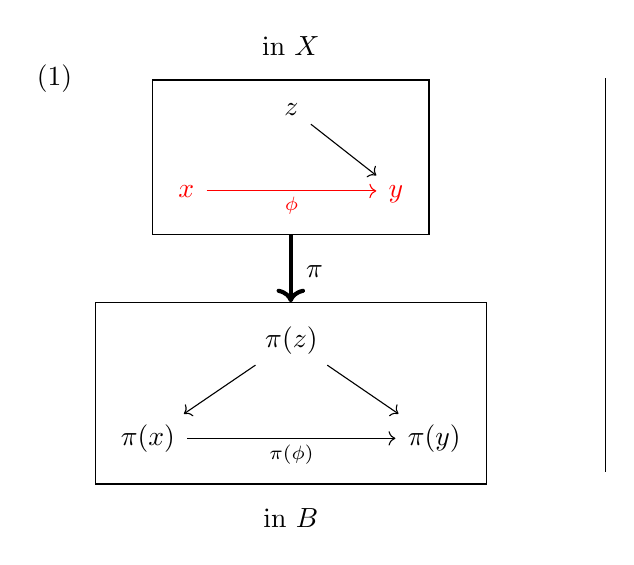
\begin{tikzpicture}[mybox/.style={draw, inner sep=5pt}]
    \node[mybox] (X) at (0,3){%
        \begin{tikzcd}
            {} & z \ar[rd]& {} \\
            \color{red}x \ar[rr, red, "\phi"'] &{}& \color{red}y
        \end{tikzcd}
    };
    \node[mybox] (B) at (0,0){%
        \begin{tikzcd}
            {} & \pi(z) \ar[rd]\ar[ld]& {} \\
            \pi(x) \ar[rr, "\pi(\phi)"'] &{}& \pi(y)
        \end{tikzcd}
    };

    \node [above=5pt of X] {in $\cat{X}$};
    \node [below=5pt of B] {in $\cat{B}$};
    \draw [->, line width=1.5pt] (X) edge (B);
    \node at (0.3,1.55) {$\pi$};
    \draw (4,4) -- (4,-1);
    \node at (-3,4) {($1$)};
    \end{tikzpicture}
    \qquad \qquad
    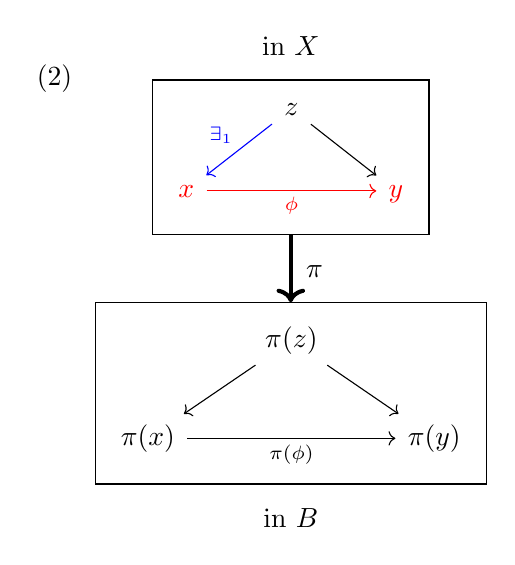
\begin{tikzpicture}[mybox/.style={draw, inner sep=5pt}]
    \node[mybox] (X) at (0,3){%
        \begin{tikzcd}
            {} & z \ar[rd] \ar[ld, blue, "\exists_1"']& {} \\
            \color{red}x \ar[rr, red, "\phi"'] &{}& \color{red}y
        \end{tikzcd}
    };
    \node[mybox] (B) at (0,0){%
        \begin{tikzcd}
            {} & \pi(z) \ar[rd]\ar[ld]& {} \\
            \pi(x) \ar[rr, "\pi(\phi)"'] &{}& \pi(y)
        \end{tikzcd}
    };

    \node [above=5pt of X] {in $\cat{X}$};
    \node [below=5pt of B] {in $\cat{B}$};
    \draw [->, line width=1.5pt] (X) edge (B);
    \node at (0.3,1.55) {$\pi$};
    \node at (-3,4) {($2$)};
    \end{tikzpicture}
    \end{center}
    %% }}}

\item
    $y \in \cat{X}, u \to \pi(y) \in \cat{B}$に対し,
    以下の図式を満たす
    \footnote{すなわち,$\pi(x)=u, \pi(x \to y)=u \to \pi(y)$を満たす.}
    \underline{$x \in \cat{X}$とcartesian arrow :: $x \to y \in \cat{X}$}を,
    cartesian lifting(or cleavage) of $u \to \pi(y)$と呼ぶ.
    \begin{center}
    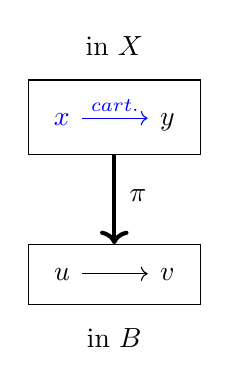
\begin{tikzpicture}[mybox/.style={draw, inner sep=5pt}]
    \node[mybox] (X) at (0,2){%
    \begin{tikzcd}
        \color{blue}x \ar[r, blue, "\text{cart.}"]& y
    \end{tikzcd}
    };
    \node[mybox] (B) at (0,0){%
    \begin{tikzcd}
        u \ar[r]& v
    \end{tikzcd}
    };

    \node [above=5pt of X] {in $\cat{X}$};
    \node [below=5pt of B] {in $\cat{B}$};
    \draw [->, line width=1.5pt] (X) edge (B);
    \node at (0.3,1) {$\pi$};
    \end{tikzpicture}
    \end{center}

\item
    任意の$y \in \cat{X}$と$u \to \pi(y) \in \cat{B}$に対してcartesian liftingが存在する
    $\pi \colon \cat{X} \to \cat{B}$をfibered categoryという.
    fibered category over $\cat{B}$が成す圏を$\Fib{B}$とする.

\item
    二つのfibered category :: 
    $\pi \colon \cat{X} \to \cat{B}, \pi' \colon \cat{X}' \to \cat{B}$について,
    $\cat{X}$と$\cat{X}'$の間の射(morphism of fibered categories, cartesian functor)とは,
    functor :: $g \colon \cat{X} \to \cat{X}'$であって,
    $\pi, \pi'$と整合的\footnote{ すなわち$\pi' \circ g=\pi$を満たす. }であり,
    cartesian arrowをcartesian arrowに写すもの.

\item
\end{myenum}
\end{Def}

\begin{Remark}
    少し圏論の言葉を整理しておく.

    対象を$0$-morphism(あるいは$0$-cell)と呼ぶ時,非負整数$k \geq 0$について,
    $k$-morphism (cell)は$(k-1)$-morphism (cell)の間の射と定義できる.
    こうして$k$-morphism (cell)は階層を成す.
    そこで,ここで定義した性質を階層別にまとめると次のように成る.
    \begin{center}
    \begin{tabular}{l|l|l}
        \hline
        arrow& arrow in a fibered category & (i) Cartesian Arrow, (ii) Cartesian Lifting \\ \hline\hline
        $0$-cell& fibered category & (iii) Existence of Cartesian Lifting \\ \hline
        $1$-cell& functor between fibered categories & (iii) Morphism of Fibered Category \\ \hline
        $2$-cell& nat. trans. between functors & (iv) Base-Preserving Natural Transformation \\
        \hline
    \end{tabular}
    \end{center}

    通常の圏同型を$1$-isoと呼び$\kiso[1]$と書く.
    この時,階層ごとのiso/equivは以下のようなものである.
    \begin{center}
        \begin{tabular}{lccl}
            iso. & $x \iso y$& $\iff$ &
                $2$つのarrow $\phi \colon x \rightleftarrows y \colon \psi$が存在し, 
                $\psi \circ \phi=\id[x], \phi \circ \psi=\id[y]$.\\ \hline\hline
            $1$-iso. & $x \kiso[1] y$& $\iff$ &
                $2$つの$1$-cell \,$\phi \colon x \rightleftarrows y \colon \psi$が存在し, 
                $\psi \circ \phi=\id[x], \phi \circ \psi=\id[y]$.\\
            $1$-equiv. & $x \kequiv[1] y$& $\iff$ &
                $2$つの$1$-cell \,$\phi \colon x \rightleftarrows y \colon \psi$が存在し, 
                $\psi \circ \phi \kiso \id[x], \phi \circ \psi \kiso \id[y]$.\\ \hline
            $2$-iso. & $x \kiso[2] y$& $\iff$ &
                $2$つの$2$-cell \,$\phi \colon x \rightleftarrows y \colon \psi$が存在し, 
                $\psi \circ \phi=\id[x], \phi \circ \psi=\id[y]$.\\
            $2$-equiv. & $x \kequiv[2] y$& $\iff$ &
                $2$つの$2$-cell \,$\phi \colon x \rightleftarrows y \colon \psi$が存在し, 
                $\psi \circ \phi \kiso[1] \id[x], \phi \circ \psi \kiso[1] \id[y]$.\\
        \end{tabular}
    \end{center}
\end{Remark}

\begin{Remark}
    $\Fib{B}$は$2$-categoryである.
    $2$-categoryは$2$-morphism ($\Fib{B}$ではnatural transformation)に
    ``vertical composition"と``horizontal composition"の二種類の合成が定まる圏である.
    詳しくはこのノートでは触れない.
\end{Remark}

\begin{Def}[Base-Preserving Natural Transformation, $\HOM$, Equivalence]
\begin{myenum}
\item
    二つのfibered category :: 
    $\pi \colon \cat{X} \to \cat{B}, \pi' \colon \cat{X}' \to \cat{B}$の間の$2$つの射
    $g,g' \colon \cat{X} \to \cat{X}'$と
    natural transformation :: $\alpha \colon g \to g'$を考える.
    \begin{center}
    \begin{tikzcd}[column sep=3cm]
        \cat{X} \ar[rd, "\pi"]\ar[dd, shift right=3mm, "g"'{name=g}] \ar[dd, shift left=3mm, "g'"{name=gg}]& {} \\
        {} & \cat{B} \\
        \cat{X}' \ar[ru, "\pi'"']& {}
        \ar[Rightarrow, from=g, to=gg, shorten >=2pt, shorten <=2pt, "\alpha"]
    \end{tikzcd}
    \end{center}
    任意の$x \in \cat{X}$について,
    $\pi'(\alpha_x) \colon \pi'(g(x)) \to \pi'(g'(x))$が恒等射になるとき,
    $\alpha$をbase-preserving natural transformationという.
    
\item
    $\cat{X}, \cat{X}' \in \Fib{B}$について,
    $\HOM_{\cat{B}}(\cat{X}, \cat{X}')$を次の圏とする.
    \begin{description}
        \item[Object.] morphism of fibered category $\cat{X} \to \cat{X}'$.
        \item[Arrows.] base-preserving natural transformation.
    \end{description}

\item
    morphism of fibered category :: $g \colon \cat{X} \to \cat{X}'$が
    equivalence of fibered categoryであるとは,
    別のmorphism $h \colon \cat{X}' \to \cat{X}$が存在し,
    $h \circ g$と$\id[\cat{X}]$,$g \circ h$と$\id[\cat{X}']$の間に
    base-preserving isomorphismが存在すること
    \footnote{ 基本的にはcategory of equivalenceの定義と同じである. }.
    \[ h \circ g \kiso[2] \id[\cat{X}], g \circ h \kiso[2] \id[\cat{X}']. \]
    二つのfibrered categoryがequivalentであるとは,
    二つの間にequivalence of fibered categoryが存在するということである.
\end{myenum}
\end{Def}

\begin{Remark}
    $2$-morphism ($2$-cell)をbase-preserving natural transformationに制限した
    fibered categoryの圏を$\FibBP{B}$とすると,
    $\HOM$は$\Hom_{\FibBP{B}}$であるし,
    equivalence of fibered categoryは$\FibBP{B}$での$2$-isoである.
\end{Remark}

\section{Examples : Fibered Categories}
\begin{Example}
    morphism of schemes :: $f \colon X \to Y$を取る.
    この$f$に対し,$f$のpullbackが成す圏$\Pi(f)$を考えることが出来る.
    以下のように定義する.
    \begin{description}[labelindent=1cm]
        \item[Object.]
            pullback diagram :: 
            $\vcenter{\xymatrix{ P \ar[r]\ar[d]& X \ar[d]^-{f}\\ Z \ar[r]& Y \centerpb }}$.
        \item[Arrow.]
            pullback diagramと整合的な射の組$(Z \to Z', P \to P')$.
    \end{description}
    $\Pi(f)$から次のようにprojectionが定まる.
    \begin{defmap}
        \pi\colon & \Pi(f)& \to& \Sch/Y \\
        {}& \vcenter{\xymatrix{ P \ar[r]\ar[d]& X \ar[d]^-{f}\\ Z \ar[r]& Y \centerpb }}& \mapsto& [ Z \to Y ]
    \end{defmap}
    ここで注意したいのは,
    $\Pi(f)$はpullback of $f$の同型類や代表ではなく,pullback of $f$全てであることである.
    したがって$\pi \colon \Pi(f) \to \Sch/Y$は
    pullback of $f$を選択公理無しに扱う枠組を与えている.
\end{Example}

\begin{Example}
    category :: $\cat{C}$について,
    arrow category :: $\cat{C}^{\to}$を以下で定める.
    \begin{description}
        \item[Object.] $\cat{C}$の射($[x \to u]$の様に表記する).
        \item[Arrow.]
            射$[x \to u] \to [y \to v]$は
            次の図式を可換にする$x \to y, u \to v$の組: 
            $\vcenter{\xymatrix{ x \ar@{-->}[r]\ar[d]& y \ar[d]\\ u \ar@{-->}[r]& v }}$
    \end{description}
    するとCartesian Liftingは$\cat{C}$がpullbackを持つことを意味し,
    Triangle Liftingはpullbackの普遍性を意味する.
\end{Example}

\begin{Example}\label{exm:representable}
    以下の関手はfibrationである.
    \begin{defmap}
        \pi\colon & \Sch/X& \to& \Sch \\
        {}& [Y \to X]& \mapsto& Y
    \end{defmap}
\end{Example}

\section{Propositions : Fibered Categories}
\begin{Prop}[\cite{NoteGroTop} Prop3.4]
\begin{myenum}
\item
    cartesian arrowの合成はcartesian arrowである.
\item
    $\phi \colon x \to y, \psi \colon y \to z$について,
    $\psi \circ \phi, \psi$ :: cartesian arrowならば$\psi$ :: cartesian arrow.
\end{myenum}
\end{Prop}
\begin{proof}
    Triangle Liftingのみを用いて証明できる.
    簡単なので証明は省略する.
\end{proof}

    次の命題の証明はCartesian LiftingとTriangle Liftingの使い方をよく示している.
\begin{Prop}
    $\pi \colon \cat{X} \to \cat{B}$をfibered category over $\cat{B}$とする.
    $\cat{X}$の射$x \to y$は以下のような二つの射の合成$x \to z \to y$に分解できる.
    \begin{itemize}
        \item $x \to z$ :: over $\id[\pi(x)]$.
        \item $z \to y$ :: cartesian, over $\pi(x \to y)$.
    \end{itemize}
\end{Prop}
%% {{{
\begin{proof}
    $\pi(\phi)$のcartesian liftingとして以下の図式(1)の$z$と$z \to y$を得る.
    さらにTriangle Liftingにより図式(2)の通り$\id[\pi(x)]$上の射$x \to z$を得る.
    \begin{center}
    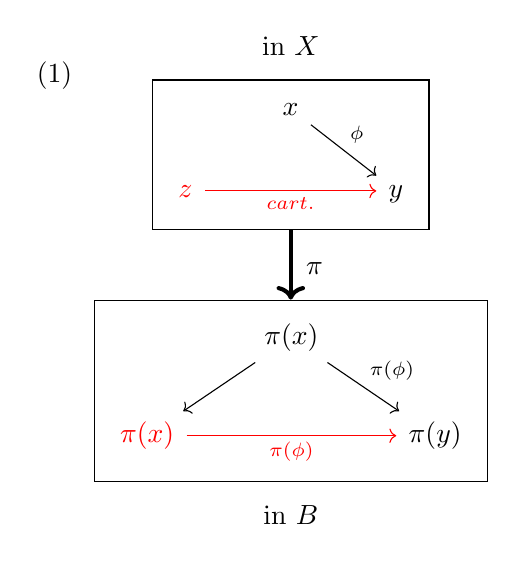
\begin{tikzpicture}[mybox/.style={draw, inner sep=5pt}]
    \node[mybox] (X) at (0,3){%
        \begin{tikzcd}
            {} & x \ar[rd, "\phi"]& {} \\
            \color{red}z \ar[rr, red, "\text{cart.}"']&{}& y
        \end{tikzcd}
    };
    \node[mybox] (B) at (0,0){%
        \begin{tikzcd}
            {} & \pi(x) \ar[rd, "\pi(\phi)"]\ar[ld, "\id"']& {} \\
            \color{red}\pi(x) \ar[rr, red, "\pi(\phi)"'] &{}& \pi(y)
        \end{tikzcd}
    };

    \node [above=5pt of X] {in $\cat{X}$};
    \node [below=5pt of B] {in $\cat{B}$};
    \draw [->, line width=1.5pt] (X) edge (B);
    \node at (0.3,1.55) {$\pi$};
%    \draw (4,4) -- (4,-1);
    \node at (-3,4) {($1$)};
    \end{tikzpicture}
    \qquad \qquad
    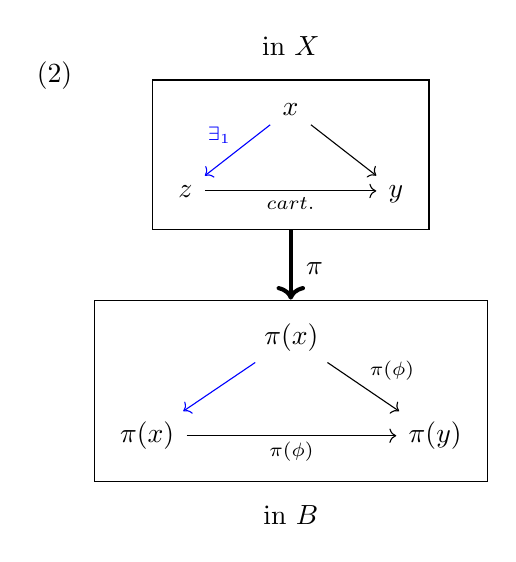
\begin{tikzpicture}[mybox/.style={draw, inner sep=5pt}]
    \node[mybox] (X) at (0,3){%
        \begin{tikzcd}
            {} & x \ar[rd] \ar[ld, blue, "\exists_1"']& {} \\
            z \ar[rr, "\text{cart.}"'] &{}& y
        \end{tikzcd}
    };
    \node[mybox] (B) at (0,0){%
        \begin{tikzcd}
            {} & \pi(x) \ar[rd, "\pi(\phi)"]\ar[ld, blue, "\id"']& {} \\
            \pi(x) \ar[rr, "\pi(\phi)"'] &{}& \pi(y)
        \end{tikzcd}
    };

    \node [above=5pt of X] {in $\cat{X}$};
    \node [below=5pt of B] {in $\cat{B}$};
    \draw [->, line width=1.5pt] (X) edge (B);
    \node at (0.3,1.55) {$\pi$};
    \node at (-3,4) {($2$)};
    \end{tikzpicture}
    \end{center}
\end{proof}
%%}}}

\begin{Prop}\label{prop:iso_over_iso}
    $\pi \colon \cat{X} \to \cat{B}$をfibered categoryとする.
    $\cat{X}$の任意のcartesian morphism :: $\phi \colon x \to y$について,
    $\phi$ :: isoと$\Phi:=\pi(\phi)$ :: isoは同値.
\end{Prop}
%% {{{
\begin{proof}
    以下の図式(1)にTriangle Liftingを用いれば,
    $\phi \circ \psi=\id[y]$なる射$\psi \colon y \to x$を得る.
    さらに図式(2)に於いて,
    $\phi \circ \id[x]=\phi=\phi \circ \psi \circ \phi$とTriangle Liftingの一意性から
    $\psi \circ \phi=\id[x]$を得る.
    \begin{center}
    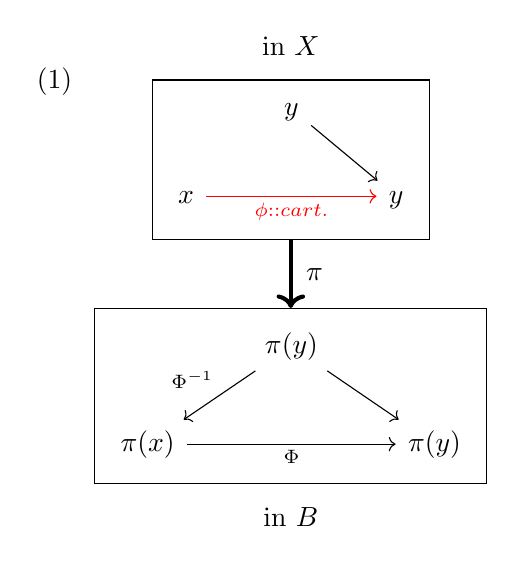
\begin{tikzpicture}[mybox/.style={draw, inner sep=5pt}]
    \node[mybox] (X) at (0,3){%
        \begin{tikzcd}
            {} & y \ar[rd, "\id"]& {} \\
            x \ar[rr, red, "\phi\text{ :: cart.}"']&{}& y
        \end{tikzcd}
    };
    \node[mybox] (B) at (0,0){%
        \begin{tikzcd}
            {} & \pi(y) \ar[rd, "\id"]\ar[ld, "\Phi^{-1}"']& {} \\
            \pi(x) \ar[rr, "\Phi"'] &{}& \pi(y)
        \end{tikzcd}
    };

    \node [above=5pt of X] {in $\cat{X}$};
    \node [below=5pt of B] {in $\cat{B}$};
    \draw [->, line width=1.5pt] (X) edge (B);
    \node at (0.3,1.55) {$\pi$};
%    \draw (4,4) -- (4,-1);
    \node at (-3,4) {($1$)};
    \end{tikzpicture}
    \qquad \qquad
    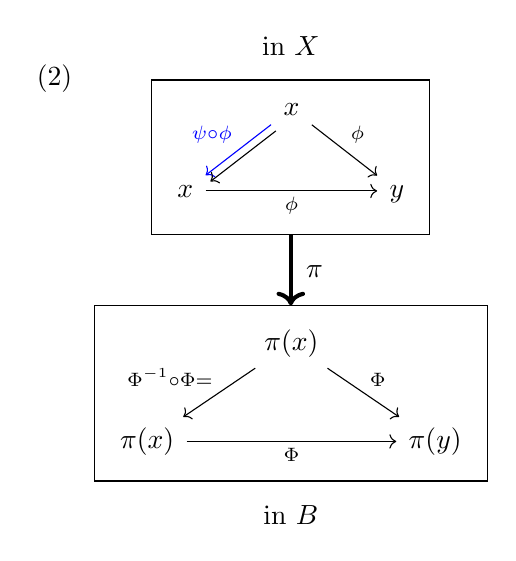
\begin{tikzpicture}[mybox/.style={draw, inner sep=5pt}]
    \node[mybox] (X) at (0,3){%
        \begin{tikzcd}
            {} & x \ar[ld, blue, "\psi \circ \phi"'] \ar[ld, shift left=1mm, "\id"] \ar[rd, "\phi"]& {} \\
            x \ar[rr, "\phi"'] &{}& y
        \end{tikzcd}
    };
    \node[mybox] (B) at (0,0){%
        \begin{tikzcd}
            {} & \pi(x) \ar[ld, "\Phi^{-1} \circ \Phi=\id"']\ar[rd, "\Phi"]& {} \\
            \pi(x) \ar[rr, "\Phi"'] &{}& \pi(y)
        \end{tikzcd}
    };

    \node [above=5pt of X] {in $\cat{X}$};
    \node [below=5pt of B] {in $\cat{B}$};
    \draw [->, line width=1.5pt] (X) edge (B);
    \node at (0.3,1.55) {$\pi$};
    \node at (-3,4) {($2$)};
    \end{tikzpicture}
    \end{center}
\end{proof}
%% }}}

\section{Fiber of Fibered Categories}
\subsection{Motivation}

\subsection{Definition}
\begin{Def}[Fiber]
    $\pi \colon \cat{X} \to \cat{B}$をfibered categoryとする.
    任意の$b \in \cat{B}$について,
    以下で定める圏を$\cat{X}_b$あるいは$\cat{X}(b)$と書き,
    fiber of $\pi$ at (over) $b$と呼ぶ:
    \begin{description}[labelindent=1cm]
        \item[Object.] $\pi(x)=b$となるobject :: $x \in \cat{X}$.
        \item[Arrow.] $\pi(\phi)=\id[b]$となるarrow :: $\phi \in \cat{X}$.
    \end{description}

    morphism of fibered category :: $g \colon \cat{X} \to \cat{Y}$から
    fiberの間に誘導される射を$g_B \colon \cat{X}_B \to \cat{Y}_B$と書く.
\end{Def}
\begin{Remark}
    標語的には次のように定義されている.
    \[
        \cat{X}_b=\cat{X}(b):=``
        \pi^{-1} \left(
        \vcenter{\xymatrix{
            b \ar@(ur,dr)^-{\id}
        }}
        \right)"
    \]
    
    また,
    morphism of schemes :: $f \colon X \to B$のfiberが
    $f^{-1}(b)$と表現されることと比較せよ。
\end{Remark}

$\cat{X}$は上で定義したfiberとcartesian liftingによって
contravariant functorに成ることが予想される.
しかしこれは一般には正しくない.
正確には,fibered categoryのfiberは一般にpsuedo-functorとなる.
このことは後に証明する.
\begin{Def}[Psuedo-functor (weak 2-functor)] \label{def:psuedofunctor}
    (以下のURLを参照せよ: \url{https://stacks.math.columbia.edu/tag/003G}.)
    $2$-圏$\cat{C}$から$2$-圏$\cat{D}$への
    psuedo-functor :: $F \colon \cat{C} \to \cat{D}$とは,
    $\cat{C}$のobjectを$\cat{D}$のobjectへ,
    $\cat{C}$のarrowを$\cat{D}$のarrowへ対応させるものであり,
    以下を満たす.
    
    \begin{enumerate}[label=(\alph*)]
        \item
            任意の$c \in \cat{C}$について
            $2$-isomorphism $\alpha_{c} \colon F(\id[c]) \to \id[F(c)]$が存在する.
        \item 任意の$f \colon c \to d, g \colon d \to e \in \cat{C}$について
            $2$-isomorphism $\alpha_{g, f} \colon F(g \circ f) \to F(g) \circ F(f)$が存在する.
        \item
            $f \colon x \to y, g \colon y \to z, h \colon z \to w$について
            以下の等式が成り立つ.
            \begin{center}
            \begin{tikzcd}[column sep=huge]
                F(x) \ar[r, bend left, "F(f)", ""{name=Fful}] \ar[r, bend right, "F(f)"', ""{name=Ffdl}]&
                F(y) \ar[r, bend left, "\id", ""{name=id}] \ar[r, bend right, "F(\id)"', ""{name=Fid}]&
                F(y)
                
                \arrow[Rightarrow, from=Fful, to=Ffdl, "\mathrm{id}_{F(f)}", shorten <=2pt]
                \arrow[Rightarrow, from=id,   to=Fid,  "\alpha_{y}", shorten <=2pt]
            \end{tikzcd}
            =
            \begin{tikzcd}[column sep=huge]
                F(x) \ar[r, bend left, "F(f)", ""{name=Ffur}]\ar[r, bend right, "F(f)"', ""{name=Ffdr}]& F(y)
                \arrow[Rightarrow, from=Ffur, to=Ffdr, "\alpha_{\mathrm{id}_y, f}", shorten <=2pt]
            \end{tikzcd}
            \end{center}
            
            \begin{center}
            \begin{tikzcd}
                F(x) \ar[r] \ar[r, bend left] \ar[rrr, bend left=40pt]& F(y) \ar[r] \ar[rr, bend left]& F(z) \ar[r]& F(w)
            \end{tikzcd}
            \end{center}
    \end{enumerate}
\end{Def}

\subsection{Propositions}
\begin{Lemma} \label{lem:cart_ump}
    $\pi \colon \cat{X} \to \cat{B}$をfibered categoryとする.
    任意の$\cat{B}$の射$f \colon b \to b'$と$x \in \cat{X}(b')$について,
    $f$と$x$に対するcartesian liftingは,
    同型を除いて一意に存在する.
\end{Lemma}
\begin{proof}
    存在はfibered categoryの定義から明らか.
    一意性はcartesian liftingが普遍性を持つことを
    Triangle Liftingを用いて示せば良い.
\end{proof}

\begin{Lemma}
    $\pi \colon \cat{X} \to \cat{B}$をfibered categoryとする.
    このとき,fiber of $\pi$はpsuedo-functorである.
\end{Lemma}
\begin{proof}
    $b \in \cat{B}$について,$\cat{X}(b)$は既に既に定義した.
    $\cat{B}$の射$\phi \colon b' \to b$について,
    関手$\cat{X}(\phi) \colon \cat{X}(b) \to \cat{X}(b')$は次のように定められる.
    まず$u \in \cat{X}(b)$について,
    $\cat{X}(\phi)(u)$は
    $\phi$による$u$のpullback :: $\phi^* u$ (cartesian lifting of $\phi$)である.
    次に$\cat{X}(b)$の射$\lambda \colon u \to v$
    ($\cat{X}(b)$の定義から$\pi(\lambda)=\id$を満たす)について,
    下の図式にtriangle liftingを用いて$\phi^*u \to \phi^*v$を得る.
    %% {{{
    \begin{center}
    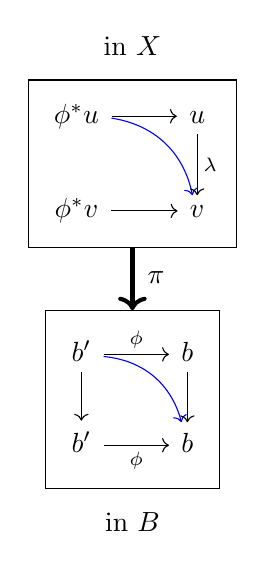
\begin{tikzpicture}[mybox/.style={draw, inner sep=5pt}]
    \node[mybox] (X) at (0,3){%
        \begin{tikzcd}
            \phi^*u \ar[r]\ar[rd, blue, bend left=35pt]& u \ar[d, "\lambda"]\\
            \phi^*v \ar[r] & v
        \end{tikzcd}
    };
    \node[mybox] (B) at (0,0){%
        \begin{tikzcd}
            b' \ar[r, "\phi"] \ar[d, "\id"']\ar[rd, blue, bend left=35pt]& b \ar[d, "\id"]\\
            b' \ar[r, "\phi"'] & b
        \end{tikzcd}
    };

    \node [above=5pt of X] {in $\cat{X}$};
    \node [below=5pt of B] {in $\cat{B}$};
    \draw [->, line width=1.5pt] (X) edge (B);
    \node at (0.3,1.55) {$\pi$};
    \end{tikzpicture}
    \end{center}
    %% }}}

    定義(\ref{def:psuedofunctor})にある条件(a)については,
    各$b \in \cat{B}$について,
    命題(\ref{prop:iso_over_iso})を用いれば同型の存在が分かる.
    条件(b)については,
    各$f \colon c \to d, g \colon d \to e \in \cat{C}$と各$b \in \cat{B}$について
    補題(\ref{lem:cart_ump})を用いれば
    $\cat{X}(g \circ f)(b) \iso \cat{X}(f) \circ \cat{B}(g)(b)$が得られる.
    あとはこの同型が自然である(すなわち自然変換を定める)ことを確かめれば良い.
\end{proof}
この事実は次のセミナーで用いる.

\begin{Thm}[$2$-Yoneda Lemma (Fibered Yoneda Lemma)]
    $\pi \colon \cat{X} \to \cat{B}$ :: fibered categoryとする.
    以下のように関手を定める.
    \begin{defmap}
        Y\colon & \cat{B}& \to& \Fib{B}\\
        {}& U& \mapsto& \cat{B}/U
    \end{defmap}
    ここで$\cat{B}/U$は例(\ref{exm:representable})にあるとおり
    fibered category over $\cat{B}$である.

    この時,圏同値$\HOM_{\cat{U}}(Y(U), \cat{X}) \to \cat{X}(U)$が成り立つ.
\end{Thm}
\begin{proof}
    (TODO)
\end{proof}

\begin{Remark}
    この定理から,$\cat{X}(U)$を「空間」$\cat{X}$の$U$-rational pointsと考えることが出来る.
    また,この定理から関手$Y$が
    $U \in \cat{B}$のfibered category over $\cat{B}$への「昇格」を与えていることが分かる.
\end{Remark}

\begin{Cor}
    圏同値$U, V \in \cat{B}$について$Y(U) \simeq Y(V)$と$U \iso V$は同値.
\end{Cor}

\bibliographystyle{jplain}
\bibliography{reference}
\end{document}
